\documentclass[tikz,border=4pt]{standalone}
\usepackage{amsmath}
\usetikzlibrary{arrows.meta,positioning,calc,fit}

\begin{document}
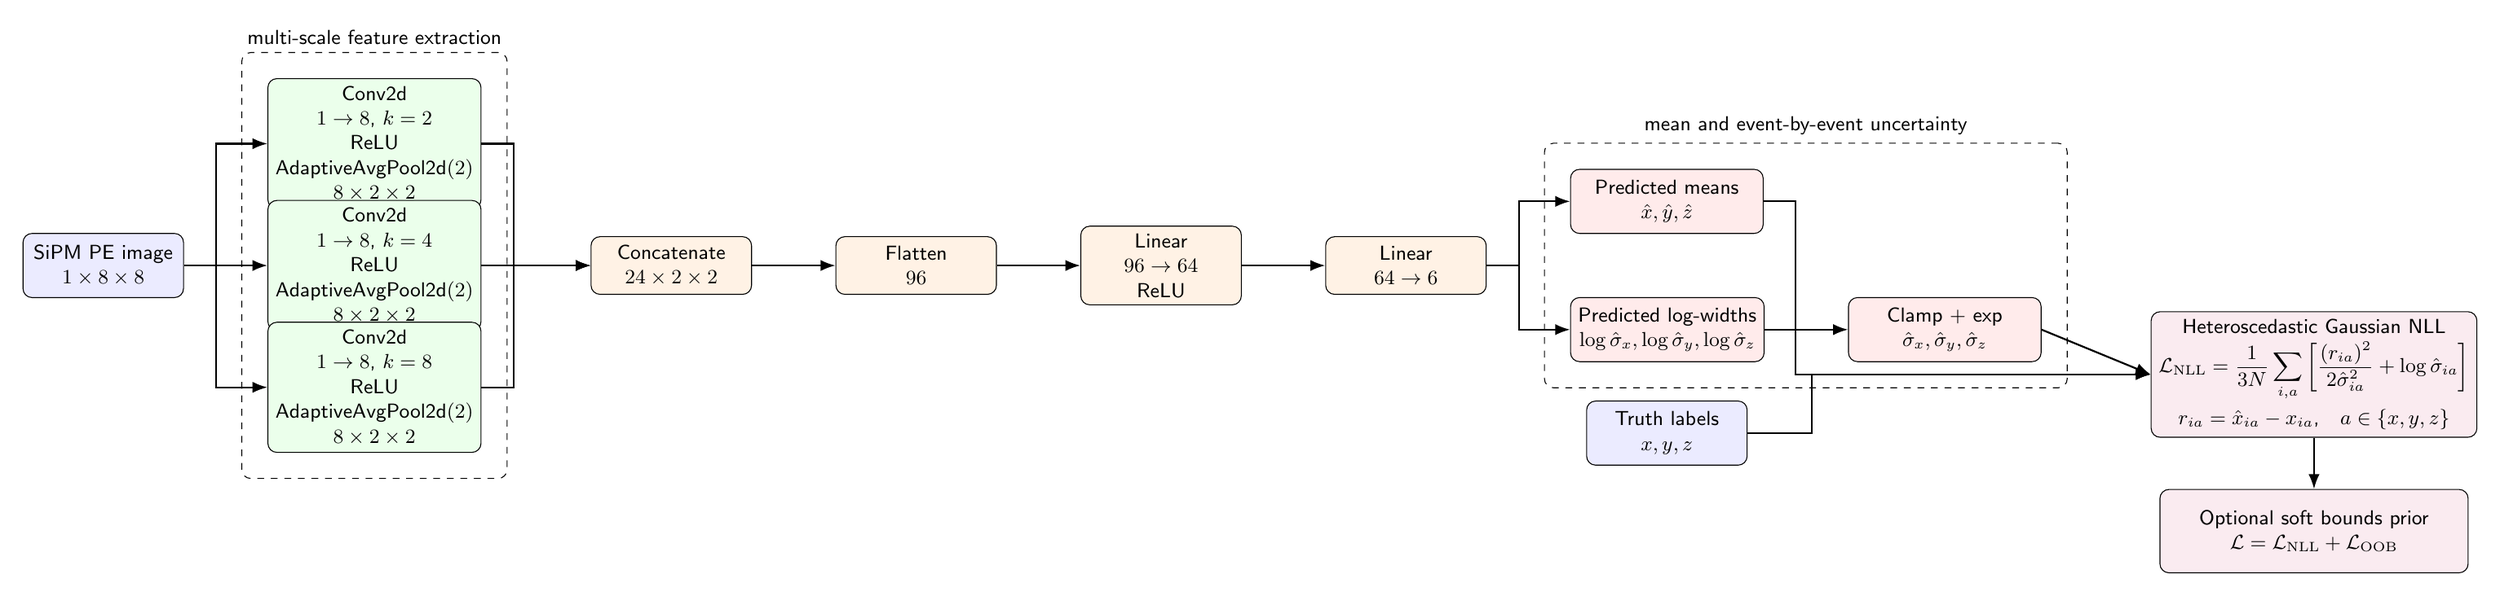
\begin{tikzpicture}[
  font=\sffamily\small,
  >=Latex,
  node distance=8mm and 13mm,
  block/.style={draw, rounded corners, align=center, minimum height=10mm, minimum width=25mm, fill=blue!8},
  branch/.style={draw, rounded corners, align=center, minimum height=13mm, minimum width=33mm, fill=green!8},
  op/.style={draw, rounded corners, align=center, minimum height=9mm, minimum width=25mm, fill=orange!10},
  output/.style={draw, rounded corners, align=center, minimum height=10mm, minimum width=30mm, fill=red!8},
  loss/.style={draw, rounded corners, align=center, minimum height=13mm, minimum width=48mm, fill=purple!8},
  arrow/.style={->, thick}
]

% Input
\node[block] (input) {SiPM PE image\\$1 \times 8 \times 8$};

% Multi-scale convolution branches
\node[branch, right=of input, yshift=19mm] (k2) {
  Conv2d\\$1 \rightarrow 8$, $k=2$\\
  ReLU\\AdaptiveAvgPool2d$(2)$\\
  $8 \times 2 \times 2$
};
\node[branch, right=of input] (k4) {
  Conv2d\\$1 \rightarrow 8$, $k=4$\\
  ReLU\\AdaptiveAvgPool2d$(2)$\\
  $8 \times 2 \times 2$
};
\node[branch, right=of input, yshift=-19mm] (k8) {
  Conv2d\\$1 \rightarrow 8$, $k=8$\\
  ReLU\\AdaptiveAvgPool2d$(2)$\\
  $8 \times 2 \times 2$
};

\draw[arrow] (input.east) -- ++(5mm,0) |- (k2.west);
\draw[arrow] (input.east) -- (k4.west);
\draw[arrow] (input.east) -- ++(5mm,0) |- (k8.west);

% Head
\node[op, right=17mm of k4] (concat) {Concatenate\\$24 \times 2 \times 2$};
\node[op, right=of concat] (flatten) {Flatten\\$96$};
\node[op, right=of flatten] (dense64) {Linear\\$96 \rightarrow 64$\\ReLU};
\node[op, right=of dense64] (dense6) {Linear\\$64 \rightarrow 6$};

\draw[arrow] (k2.east) -- ++(5mm,0) |- (concat.west);
\draw[arrow] (k4.east) -- (concat.west);
\draw[arrow] (k8.east) -- ++(5mm,0) |- (concat.west);
\draw[arrow] (concat) -- (flatten);
\draw[arrow] (flatten) -- (dense64);
\draw[arrow] (dense64) -- (dense6);

% Split outputs
\node[output, right=of dense6, yshift=10mm] (mean) {
  Predicted means\\
  $\hat{x},\hat{y},\hat{z}$
};
\node[output, right=of dense6, yshift=-10mm] (logsigma) {
  Predicted log-widths\\
  $\log \hat{\sigma}_x,\log \hat{\sigma}_y,\log \hat{\sigma}_z$
};
\node[output, right=of logsigma] (sigma) {
  Clamp + exp\\
  $\hat{\sigma}_x,\hat{\sigma}_y,\hat{\sigma}_z$
};

\draw[arrow] (dense6.east) -- ++(5mm,0) |- (mean.west);
\draw[arrow] (dense6.east) -- ++(5mm,0) |- (logsigma.west);
\draw[arrow] (logsigma) -- (sigma);

% Truth and loss
\node[block, below=26mm of mean] (truth) {Truth labels\\$x,y,z$};
\node[loss, right=17mm of sigma, yshift=-7mm] (nll) {
  Heteroscedastic Gaussian NLL\\[1mm]
  $\displaystyle
  \mathcal{L}_{\mathrm{NLL}}
  =
  \frac{1}{3N}\sum_{i,a}
  \left[
  \frac{(r_{ia})^2}{2\hat{\sigma}_{ia}^{2}}
  + \log \hat{\sigma}_{ia}
  \right]$\\[1mm]
  $r_{ia}=\hat{x}_{ia}-x_{ia}$,\quad $a\in\{x,y,z\}$
};
\node[loss, below=of nll] (oob) {
  Optional soft bounds prior\\
  $\mathcal{L}=\mathcal{L}_{\mathrm{NLL}}+\mathcal{L}_{\mathrm{OOB}}$
};

\draw[arrow] (mean.east) -- ++(5mm,0) |- (nll.west);
\draw[arrow] (sigma.east) -- (nll.west);
\draw[arrow] (truth.east) -- ++(10mm,0) |- (nll.west);
\draw[arrow] (nll) -- (oob);

% Notes
\node[draw, dashed, rounded corners, fit=(k2)(k4)(k8), inner sep=4mm,
      label={[align=center]above:multi-scale feature extraction}] {};
\node[draw, dashed, rounded corners, fit=(mean)(logsigma)(sigma), inner sep=4mm,
      label={[align=center]above:mean and event-by-event uncertainty}] {};

\end{tikzpicture}
\end{document}
